\section{Estado del arte}

% OSNT
\begin{frame}{The Open Source Network Tester}
  \begin{itemize}
    \item Sistema de captura y reproducción de código abierto
    \item Basado en una FPGA del mismo modelo que la empleada en este TFG
    \item Gestionada desde una interfaz sobre el propio servidor
    \item Se han identificado algunos aspectos mejorables
    \item El rendimiento puede verse limitado por la velocidad del disco
    \begin{itemize}
      \item Provee información exclusivamente de la FPGA
      \item Interfaz poco intuitiva
      \item Se maneja desde el propio servidor
    \end{itemize}
    \item Otras aplicaciones consideradas
    \begin{itemize}
      \item tcpdump/libpcap
      \item Wireshark
      \item Detect-Pro
    \end{itemize}
  \end{itemize}
\end{frame}

% OSNT - Interfaz
\begin{frame}{The Open Source Network Tester - Interfaz}
  \begin{figure}
    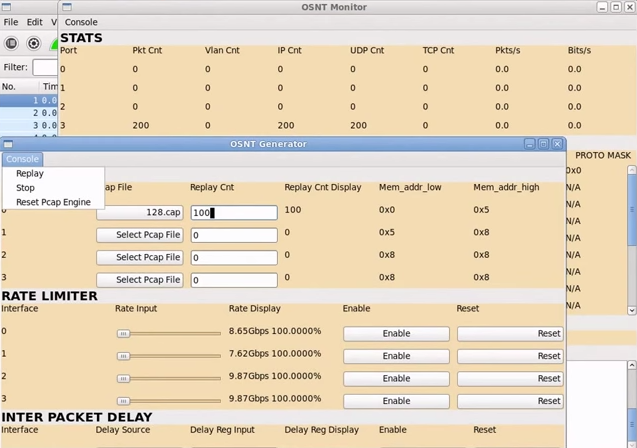
\includegraphics[width=0.9\linewidth]{osnt}
  \end{figure}
\end{frame}
